\documentclass[output=paper,
modfonts
]{langscibook} 

\title{Is the weak definite a generic? An experimental investigation} 
\author{Thaís Maíra Machado {de Sá}\affiliation{Universidade Federal de Minas Gerais}\and Greg N. Carlson\affiliation{University of Rochester}\and Maria Luiza {Cunha Lima}\affiliation{Universidade Federal de Minas Gerais}\lastand Michael K. Tanenhaus\affiliation{University of Rochester\\Nanjing Normal University}}

\ChapterDOI{10.5281/zenodo.3252028}
% \epigram{}

\abstract{We discuss the properties of \textsc{weak definite} noun phrases, \isi{definite noun phrases} (henceforth DP) which do not uniquely refer to an individual referent. Since one of the properties of \isi{generic noun phrases} is that they do not uniquely refer, we asked whether weak definites might in fact be a form of generic noun phrase. We adopted a quantitative and \is{experimental study}experimental approach conducting a corpus analysis and four experiments that were designed to assess whether weak definites differ from DPs that are generic, weak and regular definites. A corpus analysis by \citet{deSaEtAlii2016} showed that generic DPs and weak definites are not in complementary distribution. A follow-up analysis on verb \is{aktionsarten}\textit{aktionsart} showed that most weak definites appear in telic or activity DPs. The experiments also compared matched sentences with weak, regular and generic reading DPs. These studies do not find similarities between weak definites and \isi{generics}. We conclude that weak definite noun phrases are not generics.}

%\textbf{Keywords:} reference; definiteness; weak definite noun phrases; generic reference


\begin{document}
\maketitle

\section{Introduction}\label{sec:desaetal:1}\is{weak definites|(}\is{genericity|(}
Definite reference has played a central role in linguistics, the philosophy of language and in psycholinguistics \citep{Russell1905, Strawson1950,Donnellan1966,ClarkMarshall1981,Heim1982,Aguilar-GuevaraZwarts2013}. Modulo some nuanced differences in the treatment of definite reference, there is general agreement that \isi{definite noun phrases} carry a \is{familiarity}“familiarity”, \is{uniqueness|(}“uniqueness” or “identifiability” condition; the referent of a definite referring expression should be uniquely identifiable within a referential domain. In Example \REF{ex:desaetal:1}, \textit{the hospital} denotes only one hospital in the world, being \textit{unique}, and it is known by the interlocutors, being \textit{familiar}.

\ea \label{ex:desaetal:1} 
\textit{Workers picketed \textbf{the hospital} to protest layoffs.}
\z

However, so-called \textit{weak definite}\footnote{\citet{Poesio1994} was the first to use the name \textit{weak definites}, questioning the Russellian uniqueness (\citeyear{Russell1905}) and Heim’s \isi{familiarity} (\citeyear{Heim1982}). He noted that in sentences like \textit{John got these data from the student of a linguist} there is no need to have familiarity or characterize a single individual to \textit{the student} in order  to understand the sentence. He named this class of definites \textit{weak definites}. \citet{CarlsonSussman2005} adopted the \textit{weak definites} term, observing that weak definites lack uniqueness.} noun phrases \citep{CarlsonSussman2005} such as \textit{the hospital} in \REF{ex:desaetal:2} violate uniqueness: the speaker does not need to have any specific hospital in mind when she utters \textit{the hospital}. Moreover, John and Bill could even be going to different hospitals.

\ea \label{ex:desaetal:2}
\textit{John went to \textbf{the hospital} and so did Bill.}
\z

It is also known that reference in definite noun phrases can be \is{generic noun phrases}generic. In those cases, the definite noun has uniqueness of a \is{kinds}kind, i.e. it denotes a kind, not an individual referent. \textit{The hospital} in \REF{ex:desaetal:3} is an example, because it does not have an \is{uniqueness}unique individual referent, but a \is{kind reference}kind referent, \textit{the hospital} is a kind of place. 

\ea \label{ex:desaetal:3}
\textit{In the XVIII century, hygiene rules were introduced into \textbf{the hospital} in the Western world.}
\z 

For \citet[193]{Aguilar-GuevaraZwarsts2011} weak and \isi{generic definites} would be “different faces of a same phenomenon”, because both of them would have the uniqueness of a \is{kind properties}kind property, denoting a kind.  Indeed, if the lack of individual reference in weak definites can be reduced to the fact they are generic definites, it would be the most straightforward means of accounting for this lack of individual reference. 

The current work does not directly address the specific analysis proposed by \citet{Aguilar-GuevaraZwarsts2011}. Instead we address the basic question of to what extent weak definites share the properties of \isi{generic noun phrases} and regular \isi{noun phrases}.
 
In this chapter, we employ empirical means to evaluate the hypothesis that \isi{definite generics} and weak definites are the same phenomenon. We will examine corpus data form \il{Portuguese!Brazilian Portuguese}Brazilian Portuguese, and \is{experimental study}experimental data from \ili{English} to evaluate this question.

We begin with a brief summary of the properties of weak definites.


\section{Weak definites} \label{sec:desaetal:2}

The term \textit{weak definite noun phrase} is used here to describe a certain kind of construction that Carlson and collaborators (\citealt{CarlsonSussman2005,CarlsonEtAlii2006,CarlsonEtAlii2013} and \citealt{KleinEtAlii2013})
have been working on for some time under this designation. The contrasting class of \isi{definite noun phrases} is called \textit{regular definites} (sometimes “strong definites"), meaning that they trigger the \isi{familiarity}/\isi{uniqueness} presuppositions commonly focused in the literature on definite descriptions. The term \textit{weak definite noun phrase(s)} is often elided to simply \textit{weak definite(s)}, but we wish to be clear that we do not use this term in the present context to refer to just any noun phrase which, in a language differentiating \is{strong definite articles}“strong” vs \is{weak definite articles}“weak” definite article forms, has the definite article in the “weak” form.  When we wish to refer to the morphological forms of definite articles, we will do so explicitly.\is{strong definite articles}\is{weak definite articles}\is{definite articles|(}

Besides failing to trigger \is{uniqueness|)}uniqueness presuppositions, these noun phrases\linebreak, among other properties, must occur in construction with a specific verb or \is{prepositions}preposition, may only occur in the singular form or the plural form but not both, and are not subject to restrictive modification.\footnote{See \citet{Aguilar-Guevara2014} for insight into the allowable modifiers.} They appear to have the semantic truth-conditions of \is{narrow scope}narrow-scope \isi{indefinites}, and normally trigger semantically “enriching” implications -- i.e. there is a non-compositional aspect to their meaning. Finally, the constructions appear to have a more “eventive” meaning than the corresponding compositional constructions, a matter we try to pin down a bit more precisely below.\footnote{ The constructions under consideration have a number of characteristics that are summarized in \citet{CarlsonEtAlii2006}.}

Our work was motivated in part by the \is{incorporation|(}incorporation hypotheses proposed by Carlson and colleagues. Weak definite noun phrases are treated as an incorporated structure by \citet{CarlsonEtAlii2013} and \citet{KleinEtAlii2013}, in which the noun phrase and the verb have the semantics of an incorporated event in which the article, definite or \is{indefinite articles}indefinite, takes scope over the incorporated structure. This analysis unifies the observation that weak definites need not uniquely refer and the observation that they evoke habitual events associated with the noun. It also provides an explanation for the role of the definite article and makes the novel prediction that the same noun phrases that can have a weak definite interpretation can also appear in “weak indefinite” structures, which are incorporated structures that have properties more characteristic of an \is{indefinites}indefinite than a definite. Crucially this approach assumes that weak definites do not have the same properties as generic \is{definite noun phrases}DP.

In an attempt to better understand the role of the definite article in the determined phrase and in the incorporated construction, we conducted a corpus analysis and a set of \is{experimental study}experiments that examined whether weak definites exhibit properties of \isi{generics} (\sectref{seC:desaetal:3}). Then, we report the results of four experiments (\sectref{sec:desaetal:4}).

\section{Corpus analysis} \label{seC:desaetal:3}

In order to observe if weak definites would pattern with \is{generic definites|(}generic definites, \citet{deSaEtAlii2016} analyzed data on a \il{Portuguese!Brazilian Portuguese}Brazilian Portuguese (BP) corpus. Four-hundred occurrences of 31 words, which may present the weak reading in BP (e.g. \textit{the hospital}), were analyzed. They analyzed whether the word was determined by a \is{definite articles|)}definite article, and if so, whether the \is{definite noun phrases}DP reading was weak \citep{CarlsonSussman2005}, strong -- or regular -- \citep{Russell1905}, or generic \citep{Carlson2006}. They then looked at the distribution of those three kinds of definites. As expected, the regular reading is significantly more frequent than the others, 45.6\%, but surprisingly, according to the categorization criteria, the weak DPs occur significantly more often than the generic ones, 33.7\% versus 27.5\%.

The authors also described the DP’s syntactic function -- subject, object, adjunct -- for occurrences of weak, regular and generic definites in the corpus analysis. The goal was to compare the distributional properties of weak definites, generic DPs and regular definites.  They evaluated two hypotheses:
\begin{enumerate}
\item If weak definites are in fact \isi{generics},  then generic DPs and weak definites should either occur in the same environments or be in complementary distribution with one another, indicating that they are variations of the same linguistic type. \newpage
\item The second hypothesis was motivated by an analysis that weak definites undergo semantic incorporation proposed by \citet{CarlsonEtAlii2013}. The semantic incorporation hypothesis predicts that weak definites should occur primarily as the object of a verb or a \is{prepositions}preposition but rarely should occur in subject position.
\end{enumerate}


They found that \isi{generics} (\figref{fig:desaetal:1}A) are more uniformly distributed between subject (25.1\%) and object (20.3\%), being adjuncts most frequently (54.6\%). Regular definites showed the same overall pattern (\figref{fig:desaetal:1}B), presenting a significant majority of adjuncts (43.7\%), followed by objects (31.3\%), and subjects (25\%). Weak definites presented a different distribution in which they appear as adjuncts (45.7\%) as often as objects (46.6\%). Weak definites, however, seldom appear as subjects.  Only 7.2\% of the occurrences were as subjects, significantly less than the other categories (\figref{fig:desaetal:1}C).

\begin{figure}[H]
\centering
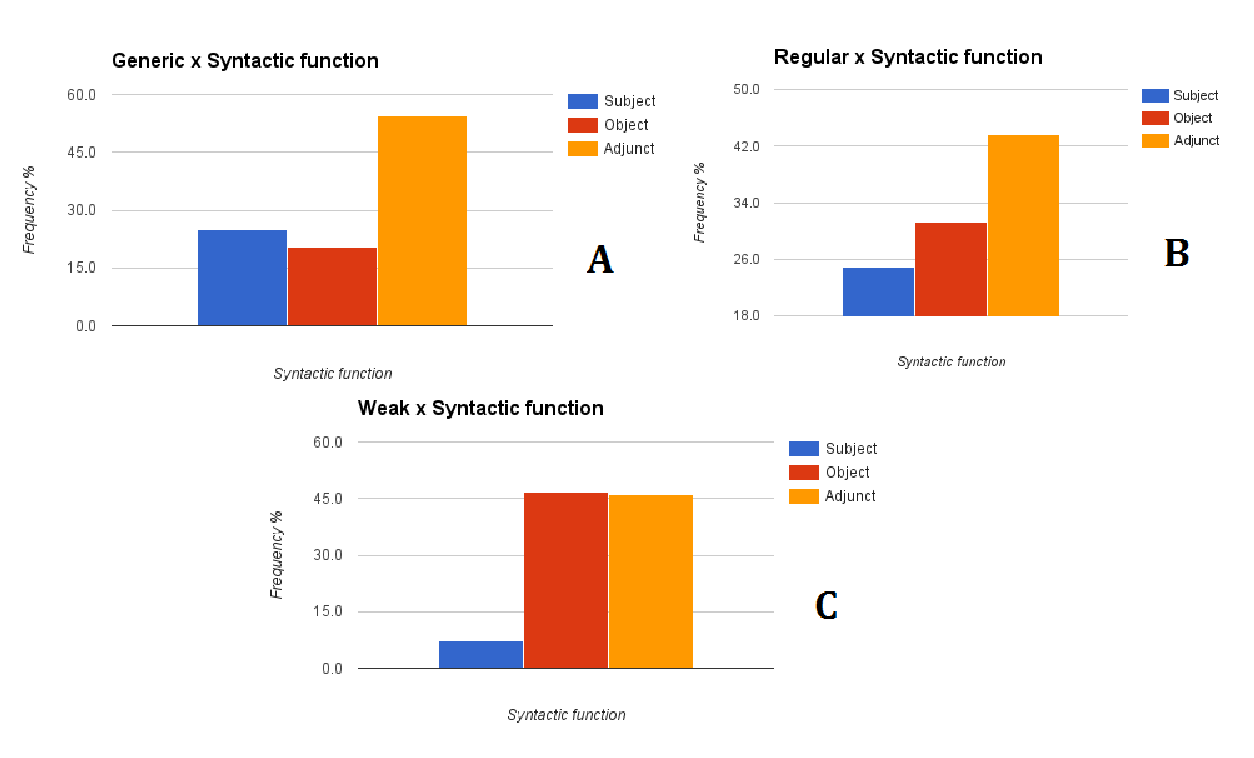
\includegraphics[width=1\textwidth]{figures/fig_tipo_sintaxe}
\caption{Definite types and syntatic function -- Generic definites (A), Regular definites (B) and Weak definites (C) \citep[114, 115]{deSaEtAlii2016}}
\label{fig:desaetal:1}
\end{figure}

The authors argued that the weak definites' high occurrence in adjunct and in object position could be interpreted as a reflex of an incorporation process, as proposed by \citet{CarlsonEtAlii2013} and \citet{KleinEtAlii2013}. But the fact that this kind of definite could also be found in subject position is a problem for the incorporation analysis. The data also did not point to a complementary distribution between weak and \is{generic definites|)}generic definites, which could be argued to provide support for the claim that they are the same phenomena.

\subsection{Aktionsarten analysis}\is{aktionsarten|(}

As a following analysis to the syntactic function analysis made by \citet{deSaEtAlii2016}, we, with the same tagged corpus, used the verb to analyze the semantics of the clause in which the \is{nouns}definite noun occurred. The verb aktionsarten\footnote{We analyzed \citet{Vendler1957} aktionsarten's categories: state, activity and telic (achievement and accomplishment).} was the semantic property we focused on motivated by the incorporation analysis, which claims that weak definites are incorporated in event or activity verbs \citep{CarlsonEtAlii2013}. 

Our hypothesis was that in aktionsart analyses, the semantic incorporation hypothesis predicts that weak definites (but not generic DPs) should primarily occur with activity and telic verbs, but not with state verbs. We also compared weak definites with \isi{generics}, which are usually found in clauses with state verbs \citep{Carlson2006}, to see if there is a complementary distribution between those categories.

For the same 2196 occurrences (of 31 words which could have generic, weak and regular readings)\footnote{Extracted from the \textit{ptTenTen} corpus, in the platform \textit{Sketch Engine}. See more information in \citet{deSaEtAlii2016}.} from \citet{deSaEtAlii2016} we analyzed the lexical aspect of the verb for the clauses containing the definite expression.

The verbs were classified as \textit{state}, \textit{activity}, or \textit{telic} (achievement and accomplishment), based on \citet{Vendler1957}. We classified as \textit{state} verbs those that do not denote an action, for example the verb \textit{ter} in \il{Portuguese!Brazilian Portuguese}BP, in the Example \REF{ex:desaetal:4}:\footnote{From here until the end of this section all the examples are from our data.} \textit{tem} does not have a process which unfolds during time, it does not denote action and if we consider its thematic role, then the subject, \textit{the school} is not an agent. 

\ea \label{ex:desaetal:4}
\il{Portuguese!Brazilian Portuguese}Brazilian Portuguese\\
\gll Além do atendimento pedagógico, a escola \textbf{tem} responsabilidades sociais. \\
Beyond {of+the} service pedagogical the school \textbf{has} responsibilities social\\  
\glt ‘The school has social responsibilities, which goes beyond the pedagogical service.’
\z

The \textit{activity} verbs are actions which do not need a conclusion point, as the verb \textit{nadar} in Example \REF{ex:desaetal:5}: \textit{nadavam} is an action that unfolds during time, but it does not have a finishing point.

\ea \label{ex:desaetal:5}
\il{Portuguese!Brazilian Portuguese}Brazilian Portuguese\\
\gll Os alunos \textbf{nadavam} todo dia na escola.\\
The students \textbf{swam} every day in+the school\\
\glt  `The students swam every day in the school.'
\z

We classified as \textit{telic} the action verbs that needed a finishing point, as \textit{quebrar}, in Example \REF{ex:desaetal:6}: \textit{quebraram} is an action that requires a conclusion point.

\ea \label{ex:desaetal:6}
\il{Portuguese!Brazilian Portuguese}Brazilian Portuguese\\
\gll Os vândalos \textbf{quebraram} a escola durante a festa.\\
The vandals \textbf{broke} the school during the party\\
\glt `Vandals broke the school during the party.'
\z

In addition to the notion of aktionsart proposed by \citet{Vendler1957}, we used the aspectual tests in \citet{Dowty1979} to distinguish one category from another in our analysis. As the Dowty tests are proposed for \ili{English}, we used a version proposed by \citet{WachowiczFoltran2006} for \il{Portuguese!Brazilian Portuguese}Brazilian Portuguese.

\subsubsection{Results}

The results are summarized in \tabref{tab:desaetal:1} and \figref{fig:desaetal:2}.

\begin{table}[H]
\centering
\caption{Weak and \isi{generic definites} and aktionsarten corpus occurrence (\%)}
\label{tab:desaetal:1}
\begin{tabularx}{.66\textwidth}{cc}
\lsptoprule
{Conditions} & {Aktionsarten corpus occurrence}                                            \\ 
\midrule
Generic                                                      & \begin{tabular}[c]{@{}c@{}}State (48.9\%)\\ Activity (37\%)\\ Telic (14.1\%)\end{tabular} \\ \\
Weak                                   &  \begin{tabular}[c]{@{}c@{}}State (16,6\%)\\ Activity (55\%)\\ Telic (28.4\%)\end{tabular}  \\ 
\lspbottomrule
\end{tabularx}
\end{table}

\begin{figure}[H]
\centering
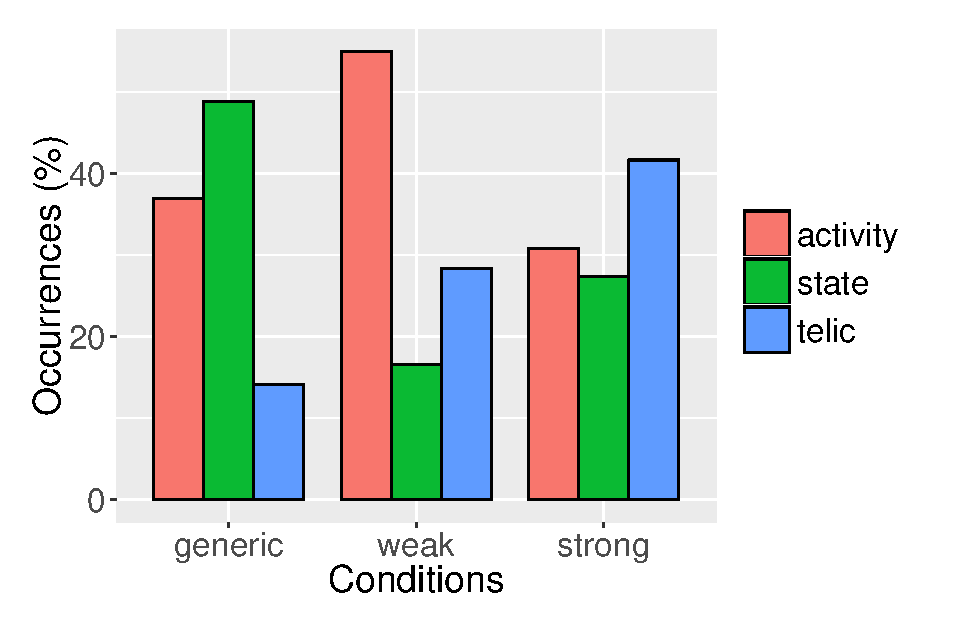
\includegraphics [width=0.8\textwidth] {figures/fig_tipo_asp}
\caption{Aktionsarten occurrence percentage in Generic, Weak and Strong conditions}
\label{fig:desaetal:2}
\end{figure}

Weak definites showed a significant difference ($\chi^2$ = 171.6676, df = 2, p < 0.001) among state, 16.6\%, activity, 55\%, and telics, 28.4\%, with activity being the most frequent category. \is{generic definites}Generic definites also significantly differ ($\chi^2$ = 85.2335, df = 2, p < 0.001) in occurrences of state, 48.9\%, telic, 14.1\%, and activity, 37\%.

The aktionsarten analysis is consistent with the incorporation hypothesis, in that weak definites are more frequent as activity and telic verbs. Also, as expected, \isi{generics} are more frequent as state verbs. One interesting finding is that weak and generic definites are not in a complementary distribution.\is{aktionsarten|)}

\subsection{Corpus summary}

The quantitative data presented in this corpus analysis introduces some interesting evidence about weak definites. Weak definites are more frequent than generic definites. Weak definites occur in subject position and they do so less frequently than in object or adjunct position. Another interesting fact about syntactic position is that there is no complementary distribution between weak and generic definites, which would have provided support for the generic hypothesis. 

The analysis of lexical aspect again found no complementary distribution between weak and generic definites. Also, as expected by the incorporation hypothesis, the majority of weak definites occur in activity and telic clauses. \is{incorporation|)}
 
\section{Experiments} \label{sec:desaetal:4}\is{experimental study|(}

We conducted four experiments in which we compared participant’s production and comprehension for stimuli that were chosen to bias weak, regular and generic readings. Our goal was to examine whether weak definites and \isi{generics} exhibited similar properties as would be predicted by the simple version of the generic hypothesis.  All of the experiments used the same materials, described in \sectref{sec:desaetal:4.1}. The experiments were conducted in \il{English!American English}American English, they were programmed in \textit{JavaScript}, and used \textit{Amazon Mechanical Turk}\footnote{Access on: \url{https://www.mturk.com/mturk/welcome}} by the software \textit{Psiturk}.\footnote{Access on: \url{https://psiturk.org/}}  We used the Mechanical Turk platform because it provides easy and fast access to participants, data collection is reliable, and results are similar to those obtained in laboratory-based experiments \citep[cf.][]{MasonSuri2012,PaolacciEtAlii2010}.


\subsection{Materials} \label{sec:desaetal:4.1}

The experimental materials were 54 sentences divided in three groups containing a \is{noun phrases}noun phrase with a \is{definite articles}definite article which had: a clear generic reading (Example \ref{ex:desaetal:7}), a clear regular reading (Example \ref{ex:desaetal:8}) and a weak reading (Example \ref{ex:desaetal:9}):


\ea \label{ex:desaetal:7}
\textit{Henry Ford created \textbf{the bus} in his early years.}
\z

\ea \label{ex:desaetal:8}
\textit{James crashed \textbf{the bus} during the night.}
\z

\ea \label{ex:desaetal:9}
\textit{Linda took \textbf{the bus} to go to college.}
\z

For all sentences, the target \is{nouns}noun was presented in a \is{definite noun phrases}definite noun phrase which was an object of a telic verb or an activity verb. In our examples, \textit{bus} is the target word, it is preceded by \textit{the}, a definite \is{determiners}determiner \textit{the bus}, in object position of a telic verb, as \textit{created}, \textit{crashed}, \textit{took}.

In Example \REF{ex:desaetal:7} the sentence in the target \is{definite noun phrases}DP has a prototypical generic reading, in which \textit{the bus}  has a \is{kinds}kind \isi{uniqueness} \citep[cf.][]{CarlsonPelletier1995,Carlson2006}. In Example \REF{ex:desaetal:8}, the \textit{the bus} has a \is{uniqueness}unique referent in the sense of \citet{Russell1905}. In  Example \REF{ex:desaetal:9}, the DP supports a weak definite reading. The weak definite sentences were modeled on examples from \citet{CarlsonSussman2005,CarlsonEtAlii2006,CarlsonEtAlii2013} and \citet{KleinEtAlii2013}.

The 54 sentences were divided into 3 lists of 18 sentences, each list with six exemplars of each type: regular, generic and weak. The same noun was never repeated within a list. The same \is{nouns}noun appeared in a different condition in each list. Each participant was presented with one of the lists. 

We briefly describe each of the four experiments in the following subsections.


\subsection{Experiment 1: Judgment}

The first experiment used a judgment task in which the participants judged\linebreak whether the \is{definite noun phrases}DP referred to either an individual or a category. We reasoned that regular \isi{definite noun phrases} would be rated as referring to individuals whereas \isi{generics} would be rated as referring to categories. Finding this pattern would provide important evidence that we had successfully created a set of materials with regular reference and a set with generic reference. The critical question was whether weak definites would pattern with the generics, as suggested by the generic hypothesis, or with regular definites. Participants read one sentence on each trial and judged if the bold word (the target word in one of the readings) was either a \textit{CATEGORY} or a \textit{INDIVIDUAL}, using a continuous scale, ranging from 0 to 100 with the words \textit{INDIVIDUAL} and \textit{CATEGORY} as the endpoints. Whether the first endpoint was individual or category was balanced within lists, as showed in the \figref{fig:desaetal:3}.

\begin{figure}[H]
\centering
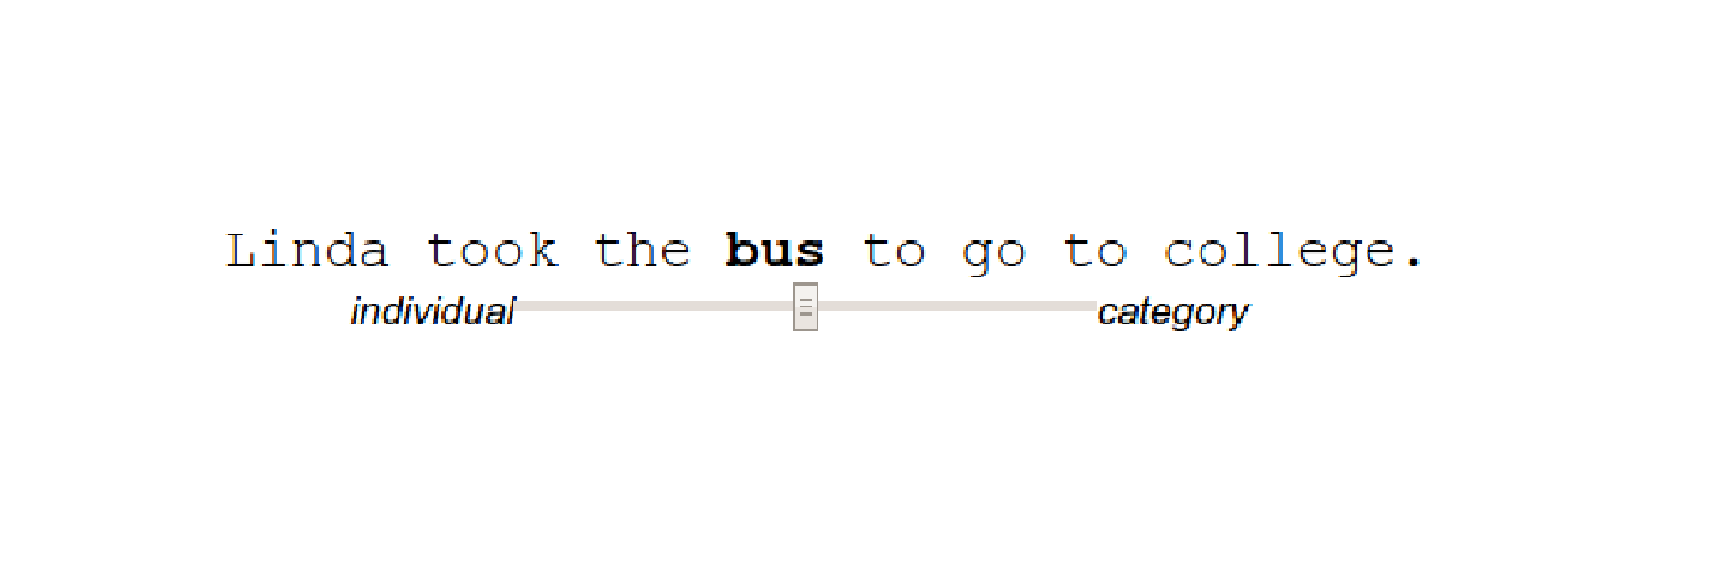
\includegraphics[width=0.9\textwidth]{figures/fig_jpinput}
\caption{Judgment task screen -- Sentence with the word \textit{bus} to be evaluated on a continuous scale (screenshot)}
\label{fig:desaetal:3}
\end{figure}

We expected that the \is{nouns}noun with a regular reading would be judged as an \textit{individual} while the generic would be evaluated as \textit{category}. This pattern of results is necessary to validate the task. The generic hypothesis predicts that the weak definites should pattern with the \isi{generic definites}, as we can see in \tabref{tab:desaetal:2}.

\begin{table}[H]\is{uniqueness}\is{kinds}
\centering
\caption{Judgment task -- Hypothesis according to generic theory}
\label{tab:desaetal:2}
\begin{tabularx}{0.66\textwidth}{c c}
\lsptoprule
{Definite readings} & {Weak = Generic}                                                         \\
\midrule
Generic                                & \begin{tabular}[c]{@{}c@{}}\textit{Category} judgment\\ (uniqueness of a kind)\end{tabular}    \\ \\
Regular                                   & \begin{tabular}[c]{@{}c@{}}\textit{Individual} judgment\\ (uniqueness)\end{tabular} \\ \\
Weak                                   & \begin{tabular}[c]{@{}c@{}}\textit{Category} judgment\\ (uniqueness of a kind)\end{tabular}    \\ \lspbottomrule
\end{tabularx}
\end{table}


\subsubsection{Participants}

90 workers (40 women) from MTurk (\url{https://www.mturk.com/}) participated for payment of US\$0.30. All participants provided informed consent in this experiment and in all of the other experiments we report. 

\subsubsection{Results}

We analyzed the data using a Linear mixed model fit by REML [`lmerMod’]. Using 0 as the individual endpoint and 100 as the category endpoint, regular definites were rated as closest to individual endpoint (mean=19.82), whereas \isi{generics} were rated as closest to the category endpoint (mean=80.63). Weak definites were rated as closer to the individual endpoint (mean=34.56). However, they fell between the regular and generics (\figref{fig:desaetal:4}). Importantly, weak definites differed significantly from both the regular and \isi{generic noun phrases} (\tabref{tab:desaetal:3}).

\begin{figure}[H]
\centering
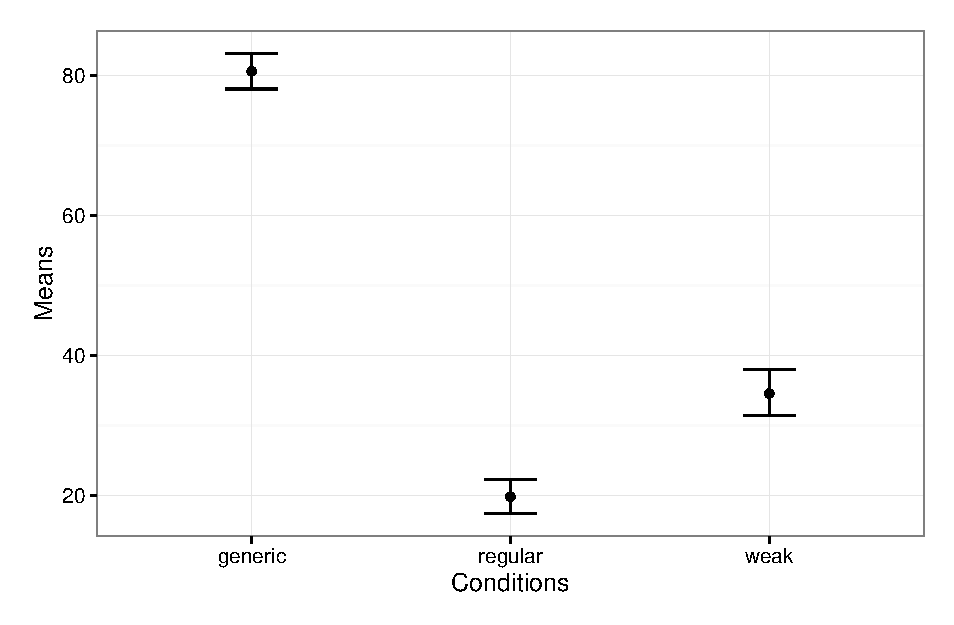
\includegraphics[width=0.8\textwidth]{figures/graf_jsmedias}
\caption{Judgment task -- Judgment means (individual to category) by condition}
\label{fig:desaetal:4}
\end{figure}

\begin{table}[H]
	\centering
	\caption{Judgment task -- Statistics -- Linear mixed model}
	\label{tab:desaetal:3}
	\begin{tabularx}{\textwidth}{cXXX}
		\lsptoprule
		\multicolumn{4}{c}{\begin{tabular}[c]{@{}c@{}}Linear mixed model fit by REML {[}`lmerMod'{]}\\ Formula: ScaledResponse $\sim$ condition + (1 + condition | subject) + (1 |,item), \\Data: data, Control: lmerControl(optimizer = ``bobyqa'')\end{tabular}} \\
		\midrule
		& { Estimate} & { Std. Error} & {t-value} \\
		\midrule
		(Intercept) & 80.561 & 2.756 & 29.24 \\ 
		Regular condition & -60.719 & 4.501 & -13.49 \\ 
		Weak condition & -46.133 & 4.134 & -11.16 \\
		\lspbottomrule
	\end{tabularx}
\end{table}

The results provide clear evidence that we successfully created two sets of sentences using the same \isi{nouns}, that when used with a \is{definite articles}definite article in a \is{definite noun phrases}DP, had a regular reading for one set and a generic reading for the second set. This serves as important validation for the materials. We also tested the prediction that if weak definites are, in fact, \isi{generics} then they would show the same pattern. However, the sentences with weak definite noun phrases did not pattern with \isi{generic noun phrases} and they were more similar to regular \isi{definite noun phrases} than they were to generics. We note, however, because judgments of weak definites fell between the regular and the generics, one could argue that weak and generic definites are not different. One characteristic of noun phrases that have weak definite readings is that they can also be interpreted as regular definites. Therefore the results for the weak definites could, in principle, reflect a mix of regular and generic interpretations. 

One way to assess the mixture possibility is to examine the distribution of responses to the three types of stimuli.  If weak definites were a mix of regular and \isi{generics}, we might expect to see a bimodal distribution, with an increased number of responses near the category endpoint. \figref{fig:desaetal:5} shows the distributions. Inspection of the patterns does not seem to support for the mixture hypothesis. Nonetheless this remains a possibility for results in which weak definites are intermediate between regulars and generics.   

\begin{figure}[H]
\centering
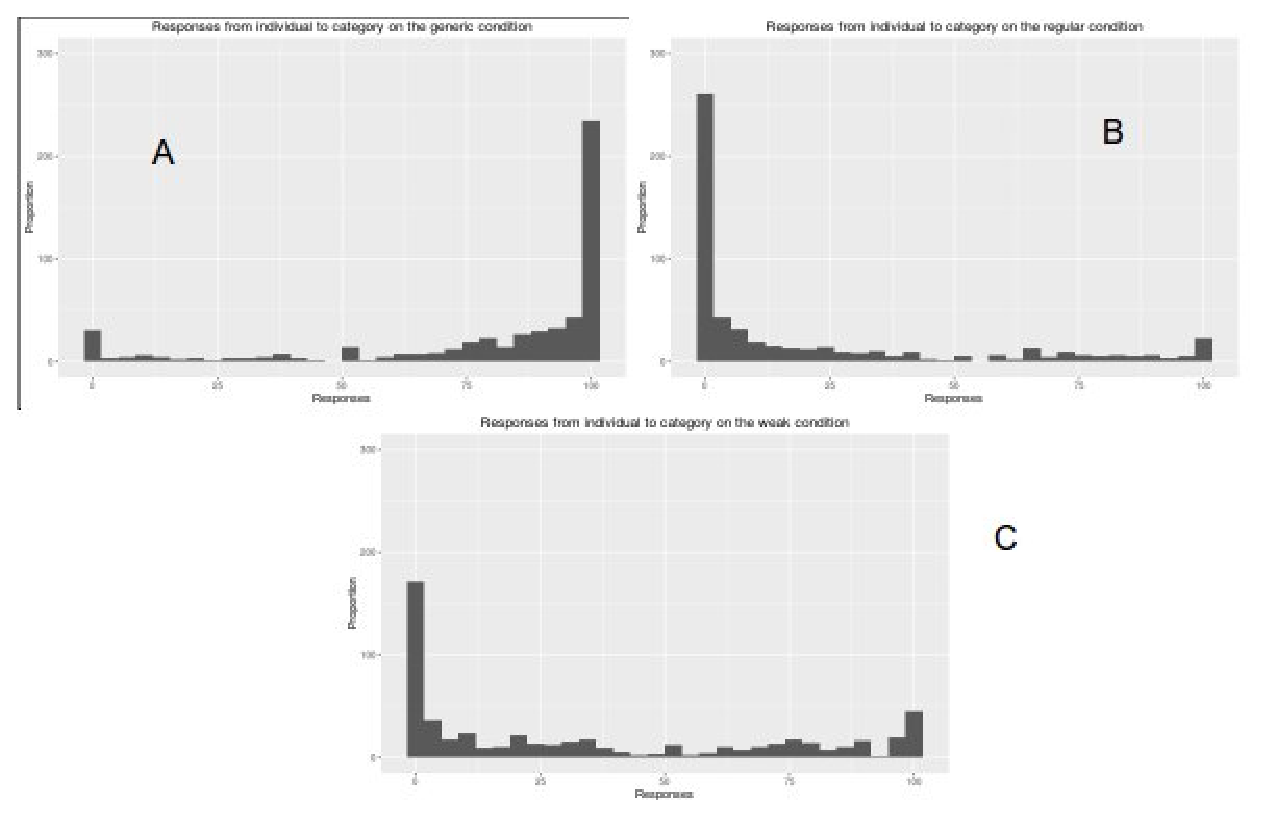
\includegraphics[width=1\textwidth]{figures/graf_hist}
\caption{Judgment task -- Condition histograms: (A) Generic distribution, (B) Regular distribution, (C) Weak distribution}
\label{fig:desaetal:5}
\end{figure}

\subsection{Experiment 2: Forced choice}

Our second experiment used a forced choice task, in which participants were presented with the same sentences as those use in the previous experiment. Participants were asked to choose between two possible \isi{noun phrases} for a continuation sentence.  One was a noun phrase that was \is{anaphora}anaphoric with the \is{definite noun phrases}definite noun phrase in the preceding sentence (e.g. \textit{That telephone...}).  The other was a\largerpage noun phrase that would introduce a new referent (e.g. \textit{A telephone...}) (Figure \ref{fig:desaetal:6}). 

\begin{figure}[H]
\centering

\includegraphics[width=0.8\textwidth]{figures/fig_fcinput}
\caption{Forced choice task screen}
\label{fig:desaetal:6}
\end{figure}

Our rationale was that regular definites would most likely be interpreted as referring to an individual, therefore licensing an \isi{anaphoric reference}.  In contrast the kind-reference supported by a generic would be more consistent with a continuation that introduced a novel referent. If weak definites are indeed a kind of generic, we would expect subjects to choose a new referent more often than the anaphoric continuation, i.e. weak definites would behave more like generic ones. 

\subsubsection{Participants}

We again tested 90 workers (34 women) from MTurk for a payment of US\$0.30, using the same lists as those created for Experiment 1. 

\subsubsection{Results}

\figref{fig:desaetal:7} and \tabref{tab:desaetal:4} show the results. As we can observe,  in sentences with the \is{generic definites}generic definite participants preferred a new referent (76.7\%), while the regular reading showed the opposite preference, with 23.4\% new referents. The weak definite did not pattern with the generic, participants chose a new referent only 42.9\% (Table \ref{table_dfstats}). 

\begin{figure}[p]
\centering
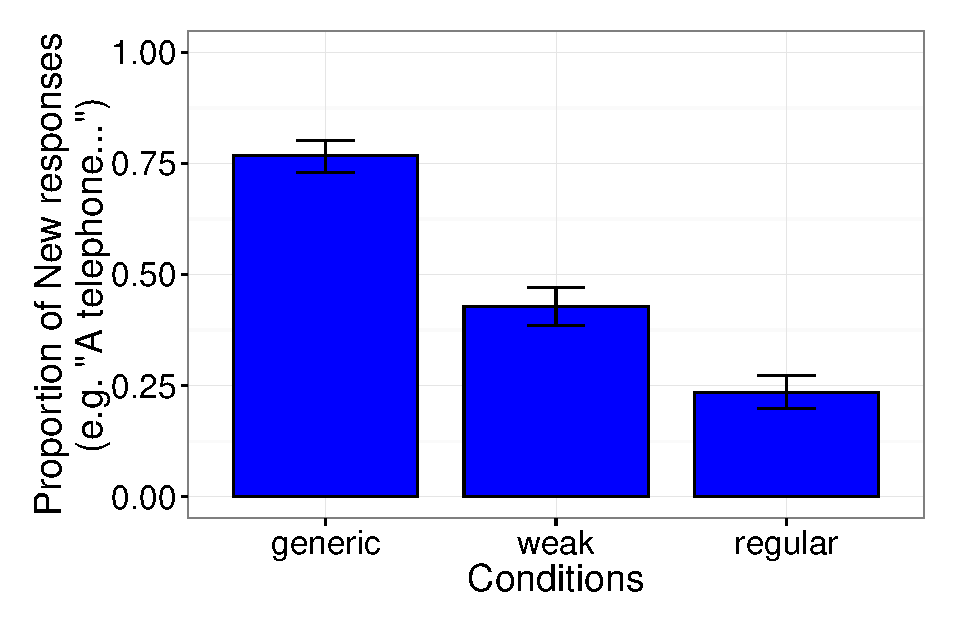
\includegraphics[width=0.7\textwidth]{figures/graf_fcnovoia}
\caption{Forced choice task -- Proportion of NEW by condition}
\label{fig:desaetal:7}
\end{figure}

\begin{table}[p]
\centering
\caption{Forced choice task -- Proportion of NEW and OLD by condition}
\label{tab:desaetal:4}
\begin{tabularx}{.60\textwidth}{ccc}
\lsptoprule
{Conditions} & {New (\textit{A X...})} & {Old (\textit{That X...)}} \\ 
\midrule
Generic & 0.767 & 0.233 \\ 
Regular & 0.234 & 0.767 \\ 
Weak & 0.429 & 0.571 \\ 
\lspbottomrule
\end{tabularx}
\end{table}

\begin{table}[p]
\centering
\caption{Forced choice task -- Generalized linear mixed model}
\label{table_dfstats}
\begin{tabularx}{\textwidth}{cXXXX}
\lsptoprule
\multicolumn{5}{c}{\begin{tabular}[c]{@{}c@{}}Generalized linear mixed model fit by maximum likelihood (Laplace \\ Approximation) \\ {[}`glmerMod'{]}, Family: binomial, ( logit )\\ Formula: choice == ``New" $\sim$ condition + (1 + condition | subject) + (1 |,item), \\ Control: glmerControl(optimizer = ``bobyqa'')\end{tabular}} \\ \midrule
 & {Estimate} & {Std. Error} & {z-value} & {Pr(\textgreater|z|)} \\ \midrule
(Intercept) & 1.4719 & 0.2118 & 6.949 & 3.67e-12 *** \\ Regular condition & -3.3248 & 0.3485 & -9.540 & \textless 2e-16 *** \\ 
Weak condition & -1.9284 & 0.3130 & -6.162 & 7.18e-10*** \\ \lspbottomrule
\end{tabularx}%
\end{table} 

Results confirmed the expected pattern both for the clearly generic and regular expressions. Although the weak definites did not pattern with the \isi{generics}, they showed fewer \is{anaphora}anaphoric choices than regular definites. This is not surprising because on the one hand, weak definites do not require a uniquely identifiable referent but, on the other hand, a weak definite noun phrase can easily be shifted to an interpretation with a uniquely identifiable referent.

Again however, one could argue that the results for weak definites could reflect a mix of generic and regular definites,  In order to provide more nuanced evidence that did not require a meta-linguistic judgment with a binary choice, we conducted two production experiments. 

\subsection{Experiment 3: Free completion} 

In this experiment participants generated continuations for the sentences used in the previous experiments. No specific constraints were put on the form of the continuations except that participants should not use language that would upset their grandparents, as in \figref{fig:desaetal:8}.


\begin{figure}[H]
\centering
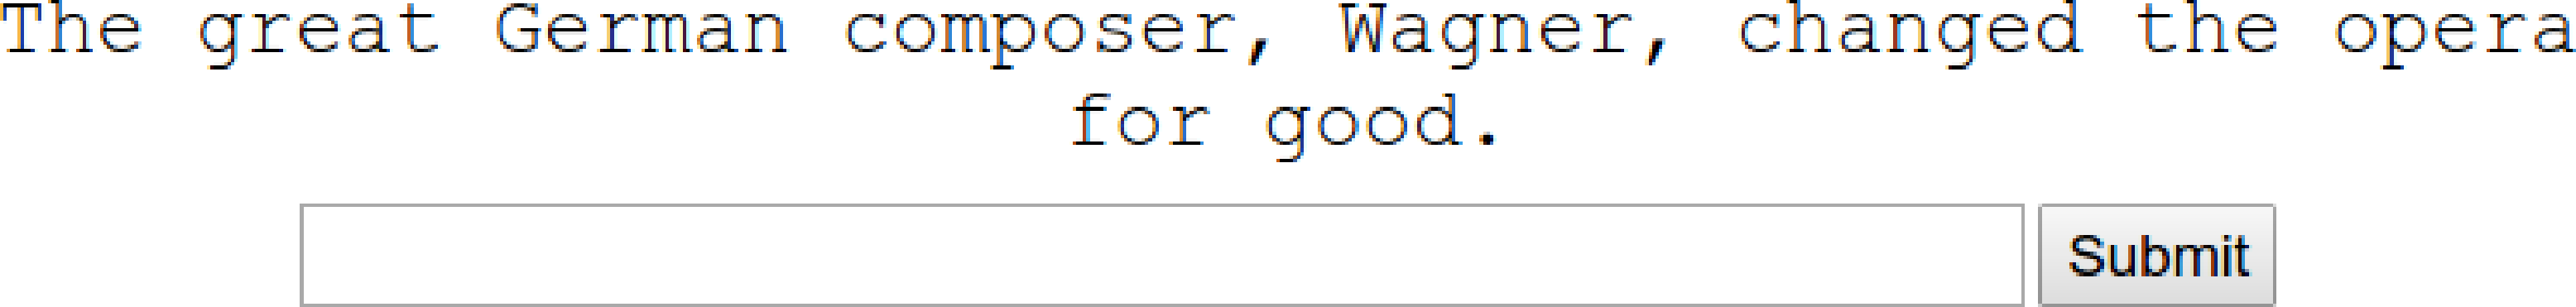
\includegraphics[width=1\textwidth]{figures/fig_compinput}
\caption{Free completion task screen}
\label{fig:desaetal:8}
\end{figure}

We analyzed the continuations to see if they repeated the definite expression. The logic of the analysis was based on the \is{incorporation}incorporation hypothesis by \citet{CarlsonEtAlii2013} and \citet{KleinEtAlii2013}. If weak definites are indeed part of incorporated structures, then the event would be more salient than an individual referent would be introduced by a regular \is{definite noun phrases}definite noun phrase or a \is{kind reference}kind-reference as introduced by a generic.

\subsubsection{Participants}
90 workers (55 men) from MTurk participated for the payment of US\$3.00. 

\subsubsection{Results}

The frequency of repetition of the target word (e.g. \textit{opera}) by condition was evaluated. The continuation in \REF{ex:desaetal:10} is an example\footnote{All the following examples are from data.} of a situation which there was no target word repetition; the experimental sentence had the target word  \textit{opera} that was not used in the completion. 

\ea \label{ex:desaetal:10}
\textbf{Experimental sentence:} \textit{The great German composer, Wagner, changed the opera for good.}
\\ \textbf{Completion:} \textit{He was a beautiful person.}
\z

We considered as repetition occurrences in which the target word was repeated in a pronoun form, as a \is{definite noun phrases}DP (any kind of \is{determiners}determiner + target word) or as a \is{bare nouns}bare noun (only the target word, on in either \is{bare plurals}plural or \is{bare singulars}singular form). In Example \REF{ex:desaetal:11}, the repetition by a pronoun form (i.e. \textit{it}) can be observed. In Example (\ref{ex:desaetal:12}), the \is{definite noun phrases}DP repetition occurred (i.e. \textit{the opera}). The last example, (\ref{ex:desaetal:13}), shows bare noun repetition (i.e. \textit{operas}).

\ea \label{ex:desaetal:11}
\textbf{Experimental sentence:} \textit{The great German composer Wagner changed the opera for good.}
\\ \textbf{Completion:} \textit{It is now much better then before.} 
\z

\ea \label{ex:desaetal:12}
\textbf{Experimental sentence:} \textit{The great German composer Wagner changed the opera for good.}	
\\ \textbf{Completion:} \textit{The opera is still a noble entertainment today.}
\z

\ea \label{ex:desaetal:13}
\textbf{Experimental Sentence:} \textit{The great German composer Wagner changed the opera for good.}
\\  \textbf{Completion:} \textit{Many later operas incorporated his changes.} 
\z

\tabref{tab:desaetal:6} and \figref{fig:desaetal:9} show that our hypothesis was confirmed, the weak definite was significantly less repeated (see Table \ref{tab:desaetal:7} for stats) than the other definite conditions.

\begin{table}[p]
\centering
\caption{Free completion task -- Proportion of target word repetition (YES) and no-repetition (NO) by condition}
\label{tab:desaetal:6}
\begin{tabularx}{0.5\textwidth}{XXX}
\lsptoprule
{Condition} & {NO} & {YES} \\
\midrule
Generic & 0.576 & 0.424 \\ 
Regular & 0.750 & 0.250 \\ 
Weak & 0.881 & 0.119 \\
\lspbottomrule
\end{tabularx}
\end{table}

\begin{figure}[p]
\centering
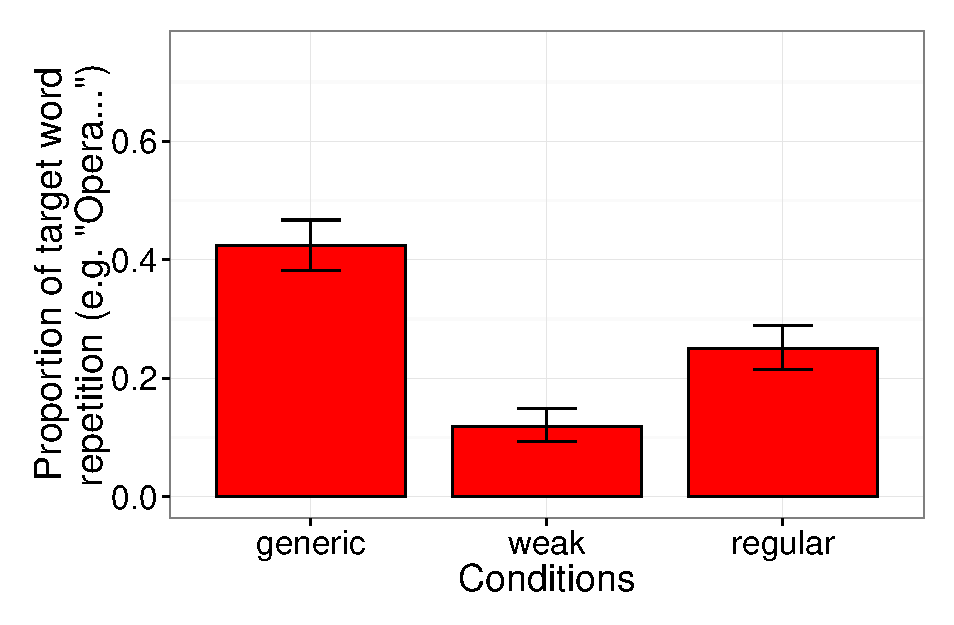
\includegraphics[width=0.7\textwidth]{figures/graf_compprop}
\caption{Free completion task -- Proportion of target word repetition by condition}
\label{fig:desaetal:9}
\end{figure}


\begin{table}[p]
\centering
\caption{Free completion task -- Generalized linear mixed model}
\label{tab:desaetal:7}
\begin{tabularx}{\textwidth}{cXXXX}
\lsptoprule
\multicolumn{5}{c}{
\begin{tabular}[c]{@{}c@{}}{\small Generalized linear mixed model fit by maximum likelihood (Laplace Approximation)}\\ {[}`glmerMod'{]}, Family: binomial, ( logit )\\ Formula: twr == ``y" $\sim$ condition + (1 | subject) + (1 |,item), Data: datac\\ Control: glmerControl(optimizer = ``bobyqa")\end{tabular}} \\ \midrule
 & {Estimate} & {Std. Error} & {z-value} & {P(\textgreater|z|)} \\ 
 \midrule
(Intercept) & -2.3662 & 0.2654 & -8.915 & \textless 2e-16 *** \\ 
Weak condition & 1.9978 & 0.3454 & 5.785 & 7.27e-09*** \\ 
Regular condition & 1.0323 & 0.3487 & 2.960 & 0.00308 ** \\ 
\lspbottomrule
\end{tabularx}
\end{table} 

The results showed that the definite noun was more likely to be repeated in a continuation for the generic and regular sentences compared to sentences with weak interpretations.  Unlike the previous studies where the weak definites fall somewhere between regular \isi{definites}, the regular and \isi{generics} were similar to one another with the weak definites showing the fewest repetitions. 

Moreover, when participants chose continuations with repetitions they tended to use different \is{morphosyntax}morphosyntactic forms and they made different semantic choices. As we can see in the occurrence examples below, (\ref{ex:desaetal:14}--\ref{ex:desaetal:16}), the experimental sentence has its target word in the generic condition in which \textit{opera} is a \is{kinds}kind. When the subjects repeated \textit{opera}, they used three different morphosyntactic forms, but they kept the kind reading.

\ea \label{ex:desaetal:14}
\textbf{Experimental sentence:} \textit{The great German composer Wagner changed the opera for good.}
\\ \textbf{Completion:} \textit{\textbf{It} is now much better then before.}
\z

\ea \label{ex:desaetal:15}
\textbf{Experimental sentence:} \textit{The great German composer Wagner changed the opera for good.}
\\ \textbf{Completion:} \textit{\textbf{The opera} is still a noble entertainment today.}
\z

\ea \label{ex:desaetal:16}
\textbf{Experimental sentence:} The great German composer Wagner changed the opera for good.	
\\  \textbf{Completion:} \textit{Many later \textbf{operas} incorporated his changes.} 
\z

The \is{morphosyntax}morphosyntactic choices for \isi{generics} was interesting, especially the use of \is{bare nouns}bare noun forms, which have a generic reading. The final experiment used a forced completion task to investigate the forms that repetition would take.


\subsection{Experiment 4: Forced completion} 
Another group of participants was asked to generate completions. In contrast to Experiment 3,  participants were instructed to repeat the bolded \is{nouns}noun used in the first sentence. However, they were not given any instructions about the form of the repetition. 

The \is{determiners}determiner choice (bare, definite, pronoun) was analyzed. We expected that, if in the first sentence there was a \is{generic definites}generic definite expression, then participants would be more likely to use the noun in a \is{bare plurals}bare plural expression compared to a regular definite. Taken as a whole, the pattern of results from the previous experiments would suggest that weak definites would show similar patterns as regular definites, with minimal use of \isi{bare nouns}.

\begin{figure}[H]
\centering
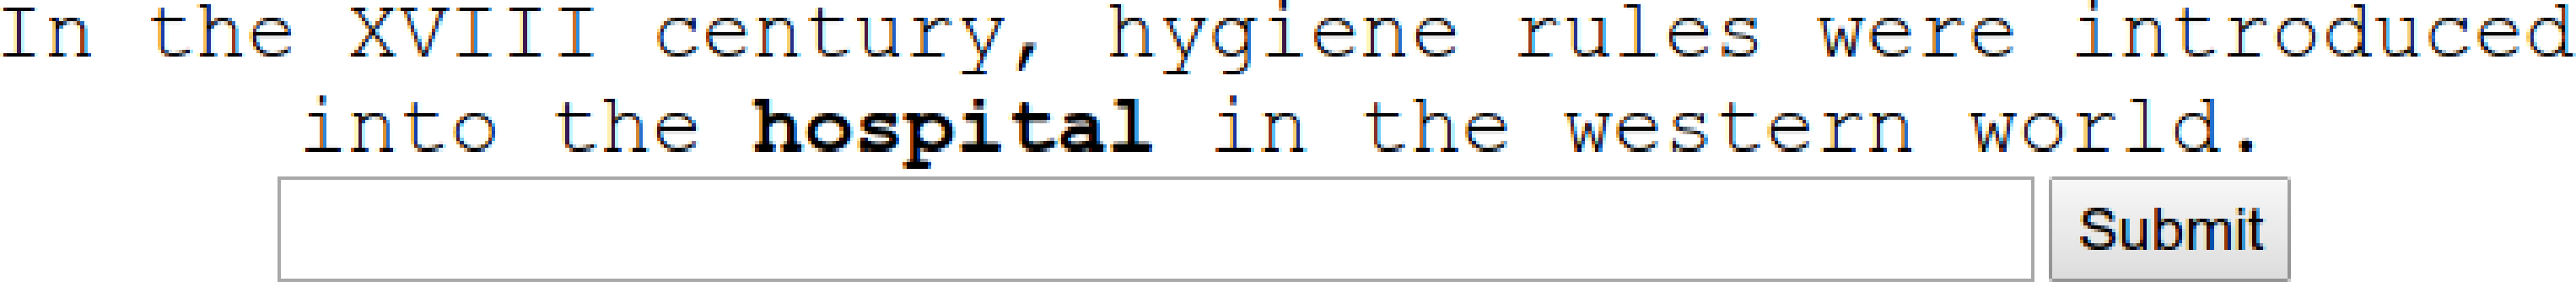
\includegraphics[width=0.9\textwidth]{figures/fig_cfinput}
\caption{Forced completion task screen}
\label{fig:desaetal:10}
\end{figure}


\subsubsection{Participants}
30 workers (16 men) from MTurk participated for the payment of US\$3.00. 

\subsubsection{Results}

In all conditions the \is{definite articles}definite article + noun \is{definite noun phrases}(“dp" in \figref{fig:desaetal:11}) was the most used form of repetition, as expected, both because the definite expression was used in the first sentence and because it is by most frequent kind of nominal phrase. However, \isi{bare plurals} were sometimes used, but only in the generic condition (“bp" in Figure \ref{fig:desaetal:11}). In fact it was the the second most preferred repetition form for the continuations following generic sentences. Crucially bare plurals were never used in continuations that followed weak definites.


\begin{figure}[H]
\centering
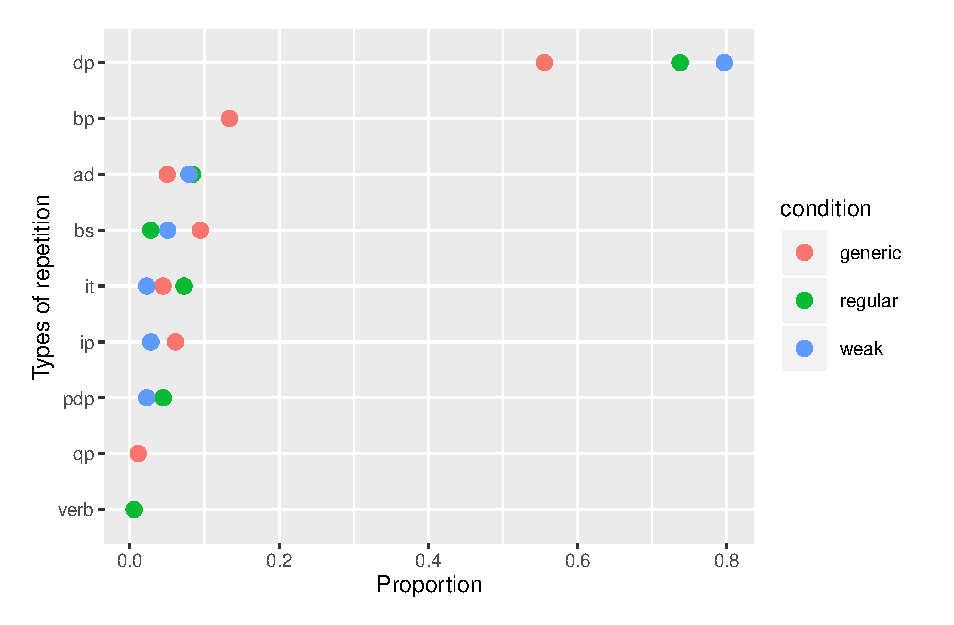
\includegraphics[width=1\textwidth]{figures/graf_cfcomo}
\caption{Forced completion -- Types of repetition by condition}
\label{fig:desaetal:11}
\end{figure}

Below there are some completions and examples of some different morphological forms of repetition founded in our data. Example \REF{ex:desaetal:17} is a \is{definite noun phrases}“dp" (the+\is{nouns}noun) occurrence; example \REF{ex:desaetal:18} a “bp" (\is{bare plurals}\is{bare nouns}bare plural noun); example \REF{ex:desaetal:19} an “ad" (noun transformed into an \is{adjectives}adjective); example \REF{ex:desaetal:20} a “verb" (noun transformed into verb).

\ea \label{ex:desaetal:17}
\textbf{Experimental sentence:} \textit{In the XVIII century hygiene rules were introduced into the	hospital in the Western world.}
\\ \textbf{Completion:} \textit{\textbf{The hospital} was now a clean place.} 
\z

\ea\label{ex:desaetal:18}
\textbf{Experimental sentence:} \textit{In the XVIII century hygiene rules were introduced into the hospital in the Western world.}
\\ \textbf{Completion:} \textit{\textbf{Hospitals} had never understood the importance of cleanliness.} 
\z

\ea \label{ex:desaetal:19}
\textbf{Experimental sentence:} \textit{In the XVIII century hygiene rules were introduced into the hospital in the Western world.}
\\ \textbf{Completion:} \textit{The \textbf{hospital} industry is now one of the largest in the world.} 
\z

\ea \label{ex:desaetal:20}
\textbf{Experimental sentence:} \textit{In Medieval times merchants used the bank to deposit their credit.}\largerpage
\\ \textbf{Completion:} \textit{Merchants did a lot of  \textbf{banking} and made money.} 
\z

Also in our data was the “bs" (\is{bare nouns}\is{bare singulars}bare noun singular), as Example \REF{ex:desaetal:21}; the pronoun (\textit{it}), Example (\ref{ex:desaetal:22}); the “ip" (noun determined by an \is{indefinite articles}indefinite article), Example \REF{ex:desaetal:23}; the “pdp" (noun determined by a pronoun), Example \REF{ex:desaetal:24}; the “qdp" (\is{nouns}noun determined by a \is{quantifiers}quantifier), Example \REF{ex:desaetal:25}.


\ea \label{ex:desaetal:21}
\textbf{Experimental sentence:} \textit{Most songwriters use the guitar when writing songs.}
\\ \textbf{Completion:} \textit{\textbf{Guitar} is the perfect instrument to work out music.} 
\z

\ea \label{ex:desaetal:22}
\textbf{Experimental sentence:} \textit{Samuel sold the guitar last year.}\footnote{\textit{Samuel vendeu a guitarra no ano passado.}}
\\ \textbf{Completion:} \textit{He didn't want to sell \textbf{it} because it was his favorite guitar but he needed the money.} 
\z

\ea \label{ex:desaetal:23}
\textbf{Experimental sentence:} \textit{Jimi Hendrix played the guitar better than anyone else.}
\\ \textbf{Completion:} \textit{Nowadays \textbf{a guitar} that was played by him is worth very much.} 
\z

\ea \label{ex:desaetal:24}
\textbf{Experimental sentence:} \textit{Zack listens to the	 radio while he drives.}
\\ \textbf{Completion:} \textit{His car \textbf{radio} is an aftermarket system.} 
\z

\ea \label{ex:desaetal:25}
\textbf{Experimental sentence:} \textit{In the XVIII century hygiene rules were introduced into the hospital in the Western world.}
\\ \textbf{Completion:} \textit{ \textbf{Every hospital} since then uses the same rules.}
\z

The \is{morphosyntax}morphosyntactic repetition form was another interesting finding which distinguishes weak and \isi{generic definites}. \is{bare nouns}\is{bare plurals}Bare plural nouns only happened in generic condition, behaving differently from weak definites once again.

\subsection{Summary of experimental findings}

In sum, we created a set of materials in which we would compare the properties of weak regular and generic sentences with object \is{definite noun phrases}DP.  Experiment 1 established that the regular and generic sentences showed the expected properties with regulars being judged as being about an individual and the \isi{generics} as about a category.  The weak definites behaved more similarly to the regular definites than the generics.  In Experiment 2 we found that, as expected, regular definites licensed \is{anaphora}anaphoric completions, whereas generics  encouraged interpretations that introduced new events.  Again weak definites behaved more similarly to regulars compared to generics.  Experiment 3 found similar results in a free completion task.  Finally, Experiment 4 required participants to repeat the \is{noun phrases}noun phrase in their completions, the distribution of the completions, suggested that generics behaved differently from both regular and weak definites.
 

\section{Conclusions} \label{sec:desaetal:5}

In this chapter we presented new data from a corpus analysis and a set of experimental studies that examined properties of weak definites, regular definites and generics. The goal of this work was to provide additional evidence that could be used to evaluate the hypothesis that weak definite noun phrases are in fact generic \is{definite noun phrases}DP. 

In a corpus analysis we found that weak definites and \isi{generics} are not in complementary distribution in either the syntactic environments in which they appear on the semantic types of events as indexed by the verb.  Moreover, as predicted by the \is{incorporation}incorporation analysis, the majority of weak definites occurred in activity and telic clauses, while \isi{generic definites} occurred more frequently in state and activity clauses. In a set of experiments we first created and validated properties of regular, generic and weak definites. We found that for the most part, weak definites behaved more like regular definites than generics. We also evaluated the possibility that the behavior of weak definites could be accounted for by the hypothesis that the behavior of weak definites reflected a mix of trials in which the weak definite was given a regular definite interpretation and trials in which it was given a generic interpretation. This type of model was, however, inconsistent with the results of several of the experiments. In sum, then, we found little evidence to support the hypotheses that weak definites showed similar properties to generics.

Our results are consistent with the incorporation hypothesis in that it assumes that the non-\isi{uniqueness} of reference in weak definites does not arise because it is a form of generic.  Therefore it would have been problematic for the incorporation hypothesis if weak definites had, in fact, patterned with generics in our studies. Further research will be necessary to determine whether the absence of generic-like behavior in these studies would be consistent with the type of analysis argued for in \citet{Aguilar-Guevara2014}, which accounts for non-uniqueness by assuming that weak definites derive their non-\isi{uniqueness} of individual reference by virtue of their generic status and their eventive properties by virtue of the KLR rules, described in detail in \citet{Aguilar-Guevara2014}.  Addressing these issues is beyond the scope of the current chapter.

Although the results we presented and the linguistic phenomena that we discussed lead us to conclude that the semantic \is{incorporation}incorporation hypothesis provides an account of the behavior of weak definites without assuming that they are \isi{generics}, it is important to conclude with some caveats. First in the corpus analysis weak definites frequently appeared in subject position, which is unexpected in the incorporation analysis. Secondly, the conclusions from our experiments bring evidence to bear on the two analyses only insofar as we have been able to tap into the relevant referential behavior with our tasks. Third, there are properties of weak definites, in particular the parallel about restrictions on modifiers for weak definites and generics, that receive a straightforward account on the generic analysis developed by \citet{Aguilar-Guevara2014}, but require additional work to be explained by the incorporation analysis.  Fourth, the arguments for the role of the \is{definite articles}definite article depend on the scoping analysis we presented, which has some precedents in the literature but is not addressed in these empirical studies.  If this analysis proves problematic, it will be important to explore other alternatives. Finally, we want to emphasize a point that has emerged from the work that the authors have conducted in collaboration with each other and with other colleagues. For a phenomenon such as weak definites which involve subtle interactions between putative structures and conceptual representations, and for which the linguistic data is less than definitive, \is{experimental study|)}experimental studies that target particular hypotheses can prove to be an important complement to linguistic argumentation.\is{weak definites|)}\is{genericity|)}

     
\section*{Acknowledgements}
This research was partially supported by NIH sentence processing grant, NIH grant HD 27206.

\section*{Abbreviations}
\begin{tabbing}
	\hspace{2.5em} \= \kill 
	BP \> \il{Portuguese!Brazilian Portuguese}Brazilian Portuguese \\
	bp \>  bare plural noun \\
	DP \>  Definite Phrase \\
	dp \>  definite article (\textit{the}) + noun \\
	ad \>  noun transformed into an \is{adjectives}adjective \\
	bs \>  bare singular noun \\
	it \>  pronoun \textit{it} \\
	ip \>  indefinite article (\textit{a}/\textit{an}) + noun \\
	pdp \>  noun determined by a pronoun \\
	qp \>  noun determined by a quantifier \\
	verb \>  noun transformed into a verb \\
\end{tabbing}

{\sloppy
\printbibliography[heading=subbibliography,notkeyword=this]
}

\end{document}

